\documentclass{article}

\usepackage{amsmath}  % To align equations
% align is from amsmath package, to allow \\ as \n and for vertical alignment

\usepackage{graphicx}
\graphicspath{ {/home/vian/0_uam/1_TFG/latex/img} }

\title{Fórmulas}
\date{}
\author{}

\begin{document}
\maketitle

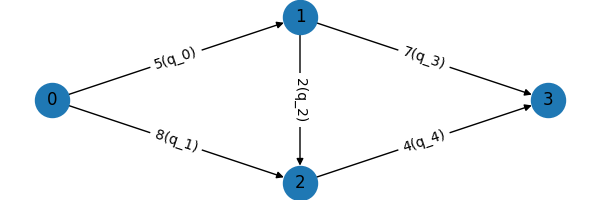
\includegraphics{primer_grafo/primer_grafo.png}

\section{Formulación del problema}

\begin{itemize}
\item \textbf{Objetivo:}
  \begin{align*}
    min(5X_{01} + 8X_{02} + 2X_{12} + 7X_{13} + 4X_{23})
  \end{align*}

\item \textbf{Restricciones:}
  \begin{align}
    & X_{01} + X_{02} = 1 \\
    & X_{01} = X_{12} + X_{13} \\
    & X_{02} + X_{12} = X_{23} \\
    & \nonumber \mathit{X_{13} + X_{23} = 1}
  \end{align}

\end{itemize}

\section{Función de coste (QUBO)}

\begin{flalign*}
  C(X) = &5X_{01} + 8X_{02} + 2X_{12} + 7X_{13} + 4X_{23} + &&\\
         &P(X_{01} + X_{02} - 1)^2 +\\
         &P(X_{01} - X_{12} - X_{13})^2 +\\
         &P(X_{02} + X_{12} - X_{23})^2
\end{flalign*}
\begin{align*}
  P = 1 + \sum_{(i, j) \in E} w_{ij} = 27
\end{align*}

\section{Correspondencia}
\begin{align*}
  X_{01} \rightarrow z_o \\
  X_{02} \rightarrow z_1 \\
  X_{12} \rightarrow z_2 \\
  X_{13} \rightarrow z_3 \\
  X_{23} \rightarrow z_4 \\
\end{align*}

\[z_a = \begin{cases}
          1 \text{ si } X_{ij} = 0 \\
          -1 \text{ si } X_{ij} = 1
        \end{cases}
      \]
      
      \[
        X_{ij} \rightarrow \frac{1 - z_a}{2}
      \]

\section{Función de coste (Ising)}

\begin{flalign*}
  C(X) \rightarrow g(z) = &5\frac{1-z_0}{2} + 8\frac{1-z_1}{2} + 2\frac{1-z_2}{2} + 7\frac{1-z_3}{2} + 4\frac{1-z_4}{2} + &&\\
                          &P(\frac{1-z_0}{2} + \frac{1-z_1}{2} - 1)^2 \\
                          &P(\frac{1-z_0}{2} - \frac{1-z_2}{2} - \frac{1-z_3}{2})^2 \\
                          &P(\frac{1-z_1}{2} + \frac{1-z_2}{2} - \frac{1-z_4}{2})^2
\end{flalign*}
\begin{flalign*}
  g(z) = &11z_0 - 17.5z_1 - 28z_2 - 17z_3 + 11.5z_4 + &&\\
         &13.5(-z_0z_2 + z_1z_2 + z_2z_3 - z_2z_4 + z_0z_1 - z_0z_3 - z_1z_4) + \\
         &(13.5z_0^2 + 13.5z_1^2 + 13.5z_2^2 + 6.75z_3^2 + 6.75z_4^2) + \\
         &26.5 = \\
         &11z_0 - 17.5z_1 - 28z_2 - 17z_3 + 11.5z_4 + \\
         &13.5(-z_0z_2 + z_1z_2 + z_2z_3 - z_2z_4 + z_0z_1 - z_0z_3 - z_1z_4) + \\
         &54 + 26.5 \\
\end{flalign*}
\begin{flalign*}
  &(z_i)^2 = 1, \forall{i \in \{-1, 1\}}&&\\
\end{flalign*}

\newpage
\section{Hamiltonian problem y mixer}
Donde \(Z\) es una puerta Pauli-Z y \(X\) una puerta Pauli-X

\begin{flalign*}
  H_p = &11Z_0 - 17.5Z_1 - 28Z_2 - 17Z_3 + 11.5Z_4 + &&\\
        &13.5(+ Z_0 \otimes Z_1 - Z_0 \otimes Z_2 - Z_0 \otimes Z_3 + Z_1 \otimes Z_2 \\
        &- Z_1 \otimes Z_4 + Z_2 \otimes Z_3 - Z_2 \otimes Z_4) + \\
        &80.5
\end{flalign*}

Debido al postulado de medición en mecánica cuántica la fase global es despreciable, por lo que
\(e^{i\gamma_i 80.5} \cdot e^{i\gamma_i H_p} = e^{i\gamma_i H_p}\).

\begin{flalign*}
  U(H_p, \gamma_i) = e^{-i \gamma_i H_p} = &Rz_0(11*2\gamma_i) \cdot Rz_1(-17.5*2\gamma_i) \cdot Rz_2(-28*2\gamma_i) \cdot Rz_3(-17*2\gamma_i) \cdot Rz_4(11.5*2\gamma_i) \cdot &&\\
                                           &Rz_0z_1(+13.5 * 2\gamma_i) \cdot Rz_0z_2(-13.5 * 2\gamma_i) \cdot Rz_0z_3(-13.5 * 2\gamma_i) \cdot Rz_1z_2(+13.5 * 2\gamma_i) \cdot \\
                                           &Rz_1z_4(-13.5 * 2\gamma_i) \cdot Rz_2z_3(+13.5 * 2\gamma_i) \cdot Rz_2z_4(-13.5 * 2\gamma_i)\\
\end{flalign*}

Pero en el paper:
\begin{flalign*}
  U(H_p, \gamma_i) = e^{-i \gamma_i H_p} = &Rz_0(11) \cdot Rz_1(-17.5) \cdot Rz_2(-28) \cdot Rz_3(-17) \cdot Rz_4(11.5) \cdot &&\\
                                           &Rz_0z_2(-13.5\gamma_i) \cdot Rz_1z_2(+13.5\gamma_i) \cdot Rz_2z_3(+13.5\gamma_i) \cdot Rz_2z_4(-13.5\gamma_i) \cdot \\
                                           &Rz_0z_1(+13.5\gamma_i) \cdot Rz_0z_3(-13.5\gamma_i) \cdot Rz_1z_4(-13.5\gamma_i) \\
\end{flalign*}

\begin{align*}
  H_m = \sum_{i=0}^{n-1}X_{i}
\end{align*}

\begin{align*}
  U(H_m, \beta_i) = e^{-i \beta_i H_m} = \prod_{i=0}^{n-1}Rx_i(2\beta_i)
\end{align*}

\subsection{Definiciones}
\begin{equation*}
  Rx_i(\lambda) = exp(-i\frac{\lambda}{2}X_i)
\end{equation*}
\begin{equation*}
  Rz_i(\lambda) = exp(-i\frac{\lambda}{2}Z_i)
\end{equation*}
\begin{equation*}
  Rz_iz_j(\lambda) = exp(-i\frac{\lambda}{2}Z_i \otimes Z_j)
\end{equation*}

\section{Hamiltonian}
\begin{itemize}
\item \textbf{Parámetros:}
  \begin{align*}
    \vec{\beta} = [\beta_0, ..., \beta_{p-1}]\\
    \vec{\gamma} = [\gamma_0, ..., \gamma_{p-1}]\\
  \end{align*}

\item \textbf{Hamiltonian}
  \begin{align*}
    H(\vec{\beta}, \vec{\gamma}) = U(H_m, \gamma_{p-1})U(H_p, \beta_{p-1}) ... U(H_m, \gamma_0)U(H_p, \beta_0)
  \end{align*}

\end{itemize}

\end{document}

%%% Local Variables:
%%% mode: latex
%%% TeX-master: t
%%% End:
